\documentclass[a4paper, amsfonts, amssymb, amsmath, reprint, showkeys, nofootinbib, twoside]{revtex4-1}
\usepackage[english]{babel}
\usepackage[utf8]{inputenc}
\usepackage[colorinlistoftodos, color=green!40, prependcaption]{todonotes}
\usepackage[pdftex, pdftitle={Article}, pdfauthor={Author}]{hyperref}
\usepackage{amsthm}
\usepackage{mathtools}
\usepackage{physics}
\usepackage{xcolor}
\usepackage{caption}
\usepackage{hyperref}
\usepackage{multirow}
\usepackage{amsmath}
\usepackage{amssymb}
\usepackage{graphicx}
\graphicspath{Images}
\usepackage[left=23mm,right=13mm,top=35mm,columnsep=15pt]{geometry} 
\usepackage{adjustbox}
\usepackage{placeins}
\usepackage[T1]{fontenc}
\usepackage{float}
%\usepackage{longtable}
\usepackage{csquotes}
\usepackage{refstyle}
\usepackage{lipsum}
\usepackage{booktabs}

\begin{document}

\title{Study of Geiger Muller Counter}
\author{Swaroop Ramakant Avarsekar}
\email{swaroop.avarsekar@niser.ac.in}
\affiliation{School of Physical Sciences, National Institute of Science Education and Research, HBNI, Jatni -752050, India}
\date{\today}

\begin{abstract}
We aim to determine the operating voltage of GM counter and hence verifying the inverse square law and calculating the efficiency of counter with gamma and beta source. We used Cs-137 as gamma source and tl-204 as beta source. In the last section, we perform nuclear counting statistics to find various parameters such as mean, variance under differnet time for background and beta source.
\end{abstract}
	
\keywords{Plataeu voltage, Dead time, Electron Avalanche, Variance}

\maketitle

\section{Theory}
Geiger Muller (GM) counters are used to detect the radioactivity. GM tube is filled with inert gas with an anode surrounded by a metal cylinder as cathode. The gas is ionized due to particles entering through window and subsequent electron movement and collision takes place resulting electron avalanche. The electrons are attracted to anode and ionized gas are attracted to cathode. The electrons from the anode flow from the power supply, resulting in counts. 

\begin{figure}[H]
	\centering
	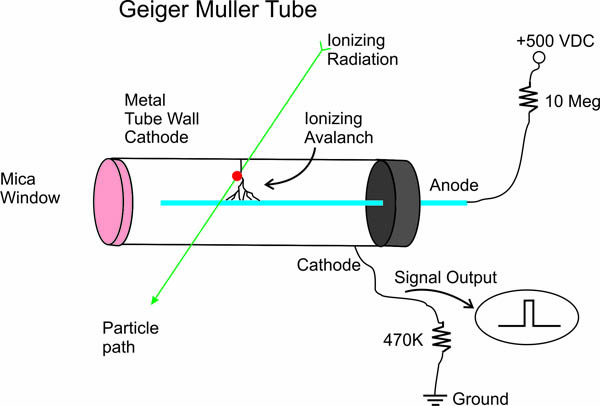
\includegraphics[scale=0.3]{gm} 
	\caption{Geiger Muller Tube}
	\label{1}
\end{figure}

Some of the terms used in GM counters are described below.
Starting voltage is lowest voltage applied to GM tube before it starts counting. Plateau is section of GM characteristic curve where count rate is independent of applied voltage. The operating voltage is mean of the plateau region. Background radiation is due to cosmic rays and other radioactive sources in the lab. Dead time ($T_d$) is time interval after initiation of discharge resulting in normal pulse where GM tube is insensitive to further ionizing events. Maximum counting rate is approximately 1/$T_d$. Recovery time is minimum time interval between two distinct ionizing events. 

Few of the sources for background radiation are the gamma radiation from the environment and cosmic radiation, mesons from cosmic radiation, beta particles from contamination, spontaneous discharge in the detector, electronic noises etc. 

\section{Experiment and Analysis}
The radioactive sources Cs-137 and Tl-204 are used as gamma and beta source, respectively throughout the experiment, as shown below.

\begin{figure}[H]
	\centering
	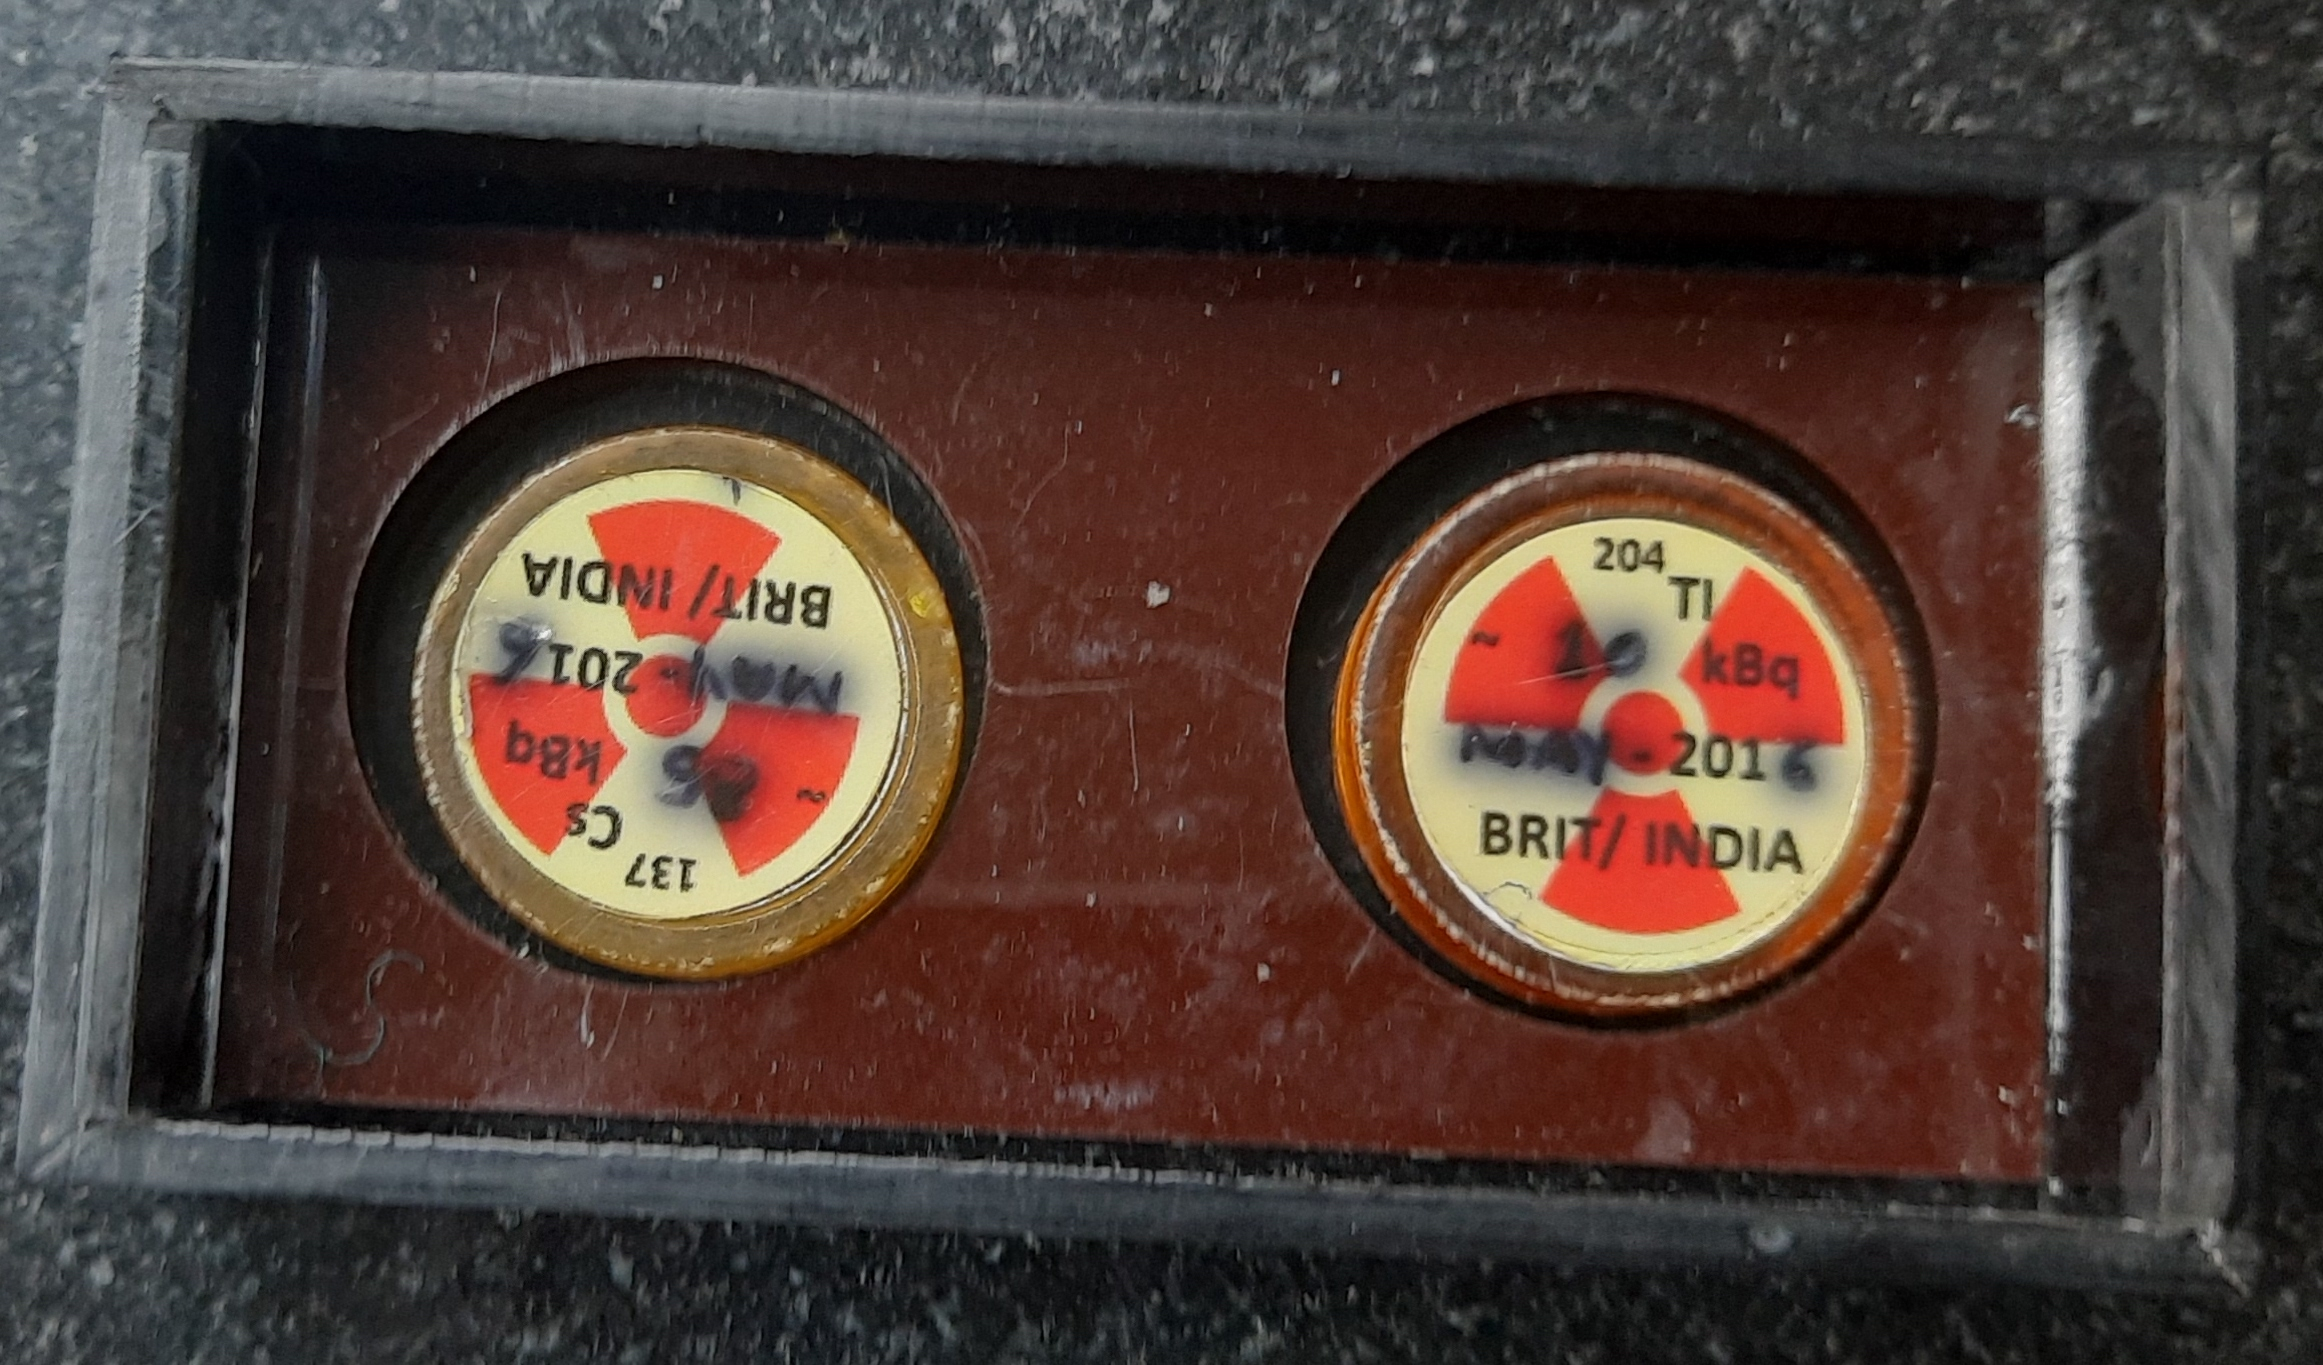
\includegraphics[scale=0.09]{source} 
	\caption{Sources Cs-137 and Tl-204 used for the experiment}
	\label{}
\end{figure}

\begin{figure}[H]
	\centering
	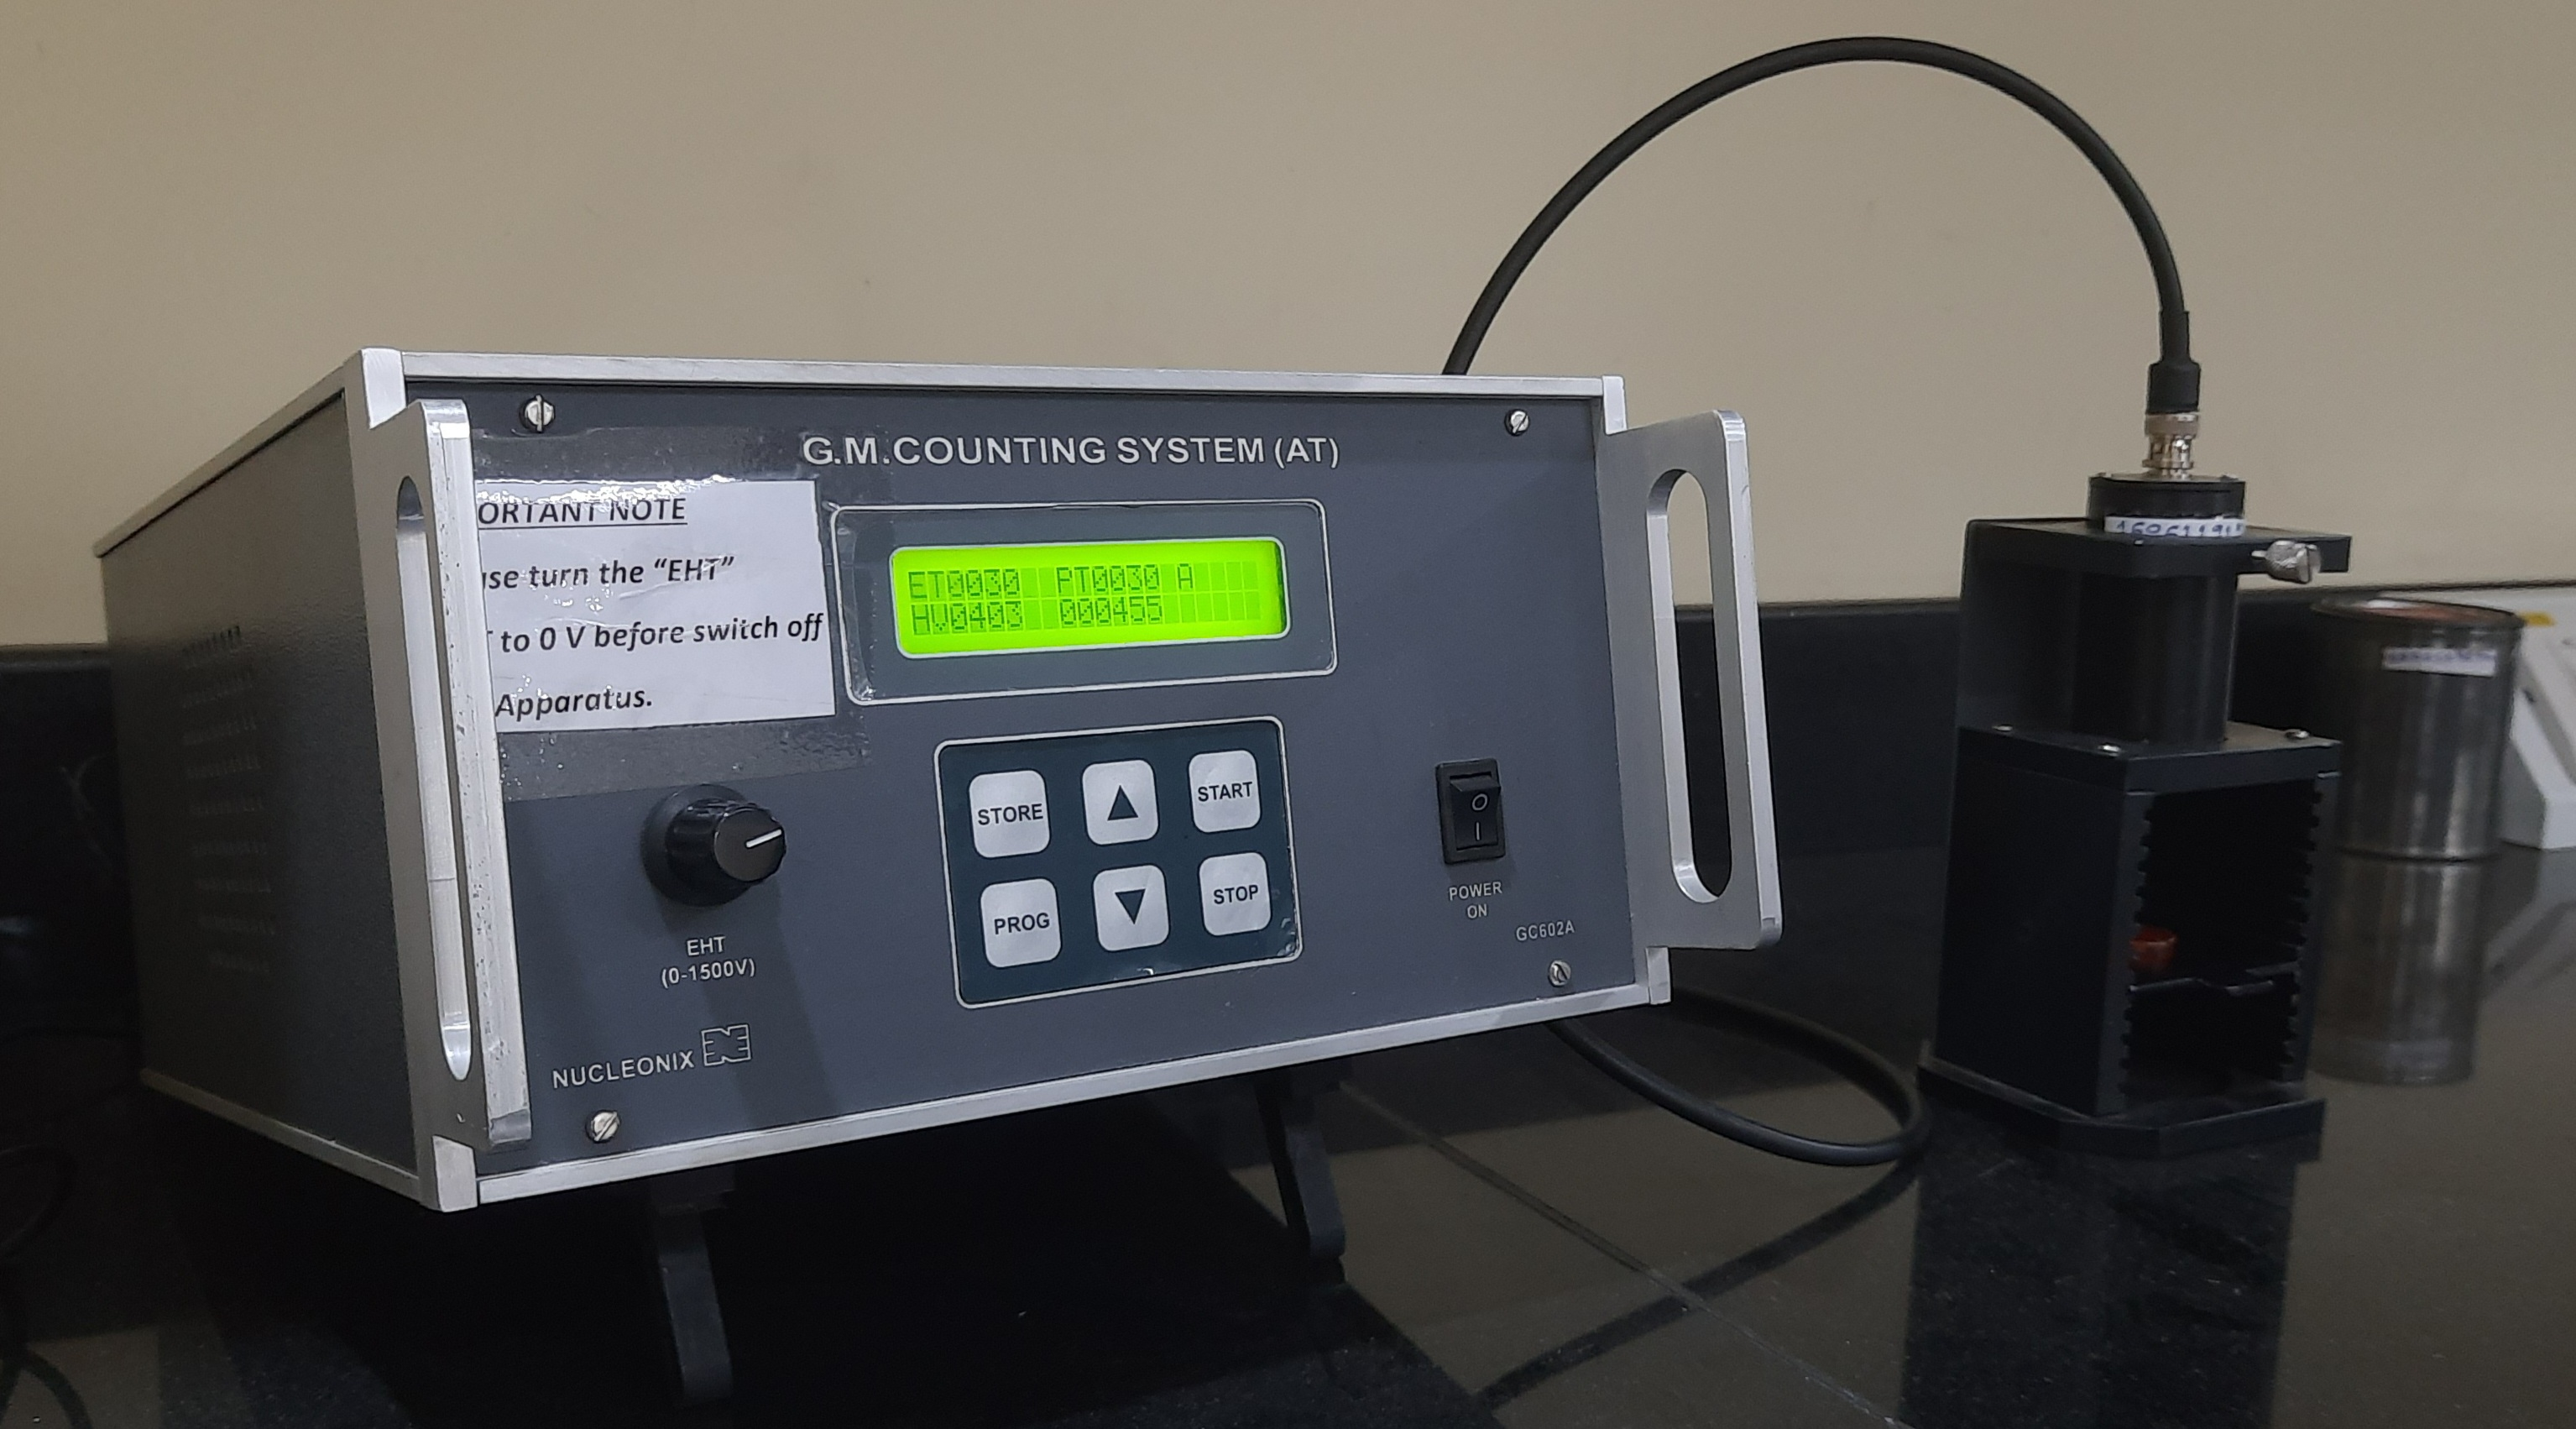
\includegraphics[scale=0.07]{gmc} 
	\caption{GM counter at lab}
	\label{}
\end{figure}

\subsection{Characteristics of GM tube}
To study the characteristics of GM tube, we determine the operating voltage with the plot of counts versus voltage. The counts are taken for 30 second time. A plateau is obtained, where the mean of plateau is the operating voltage. We also determine the plateau slope, length from this experiment. The observations are shown in table (\ref{t1}) and (\ref{t2}).

\begin{table}[H]
	\centering
	\caption{GM Characteristic Table for Cs-137}
	\label{t1}
	\resizebox{\columnwidth}{!}{%
		\begin{tabular}{|r|r|r|r|}
			\hline
			\multicolumn{1}{|l|}{HV (V)} & \multicolumn{1}{l|}{Count} & \multicolumn{1}{l|}{BG Count} & \multicolumn{1}{l|}{Corrected Count} \\ \hline
			307 & 0    & 0  & 0    \\ \hline
			337 & 2542 & 23 & 2519 \\ \hline
			367 & 2802 & 36 & 2766 \\ \hline
			397 & 2875 & 34 & 2841 \\ \hline
			427 & 2838 & 40 & 2798 \\ \hline
			457 & 2870 & 33 & 2837 \\ \hline
			487 & 2839 & 39 & 2800 \\ \hline
			517 & 3028 & 39 & 2989 \\ \hline
			547 & 2940 & 34 & 2906 \\ \hline
			577 & 2956 & 38 & 2918 \\ \hline
			607 & 3017 & 41 & 2976 \\ \hline
			637 & 4563 & 57 & 4506 \\ \hline
			667 & 5809 & 67 & 5742 \\ \hline
		\end{tabular}%
	}
\end{table}

\begin{table}[H]
	\centering
	\caption{GM Characteristic Table for Tl-204}
	\label{t2}
	\resizebox{\columnwidth}{!}{%
		\begin{tabular}{|r|r|r|r|}
			\hline
			\multicolumn{1}{|l|}{HV (V)} & \multicolumn{1}{l|}{Count} & \multicolumn{1}{l|}{BG Count} & \multicolumn{1}{l|}{Corrected Count} \\ \hline
			313 & 0   & 0  & 0   \\ \hline
			343 & 391 & 38 & 353 \\ \hline
			373 & 394 & 41 & 353 \\ \hline
			403 & 455 & 40 & 415 \\ \hline
			433 & 417 & 36 & 381 \\ \hline
			463 & 454 & 46 & 408 \\ \hline
			493 & 420 & 44 & 376 \\ \hline
			523 & 416 & 45 & 371 \\ \hline
			553 & 414 & 42 & 372 \\ \hline
			583 & 387 & 35 & 352 \\ \hline
			613 & 420 & 47 & 373 \\ \hline
			643 & 891 & 69 & 822 \\ \hline
		\end{tabular}%
	}
\end{table}

\begin{figure}[H]
	\centering
	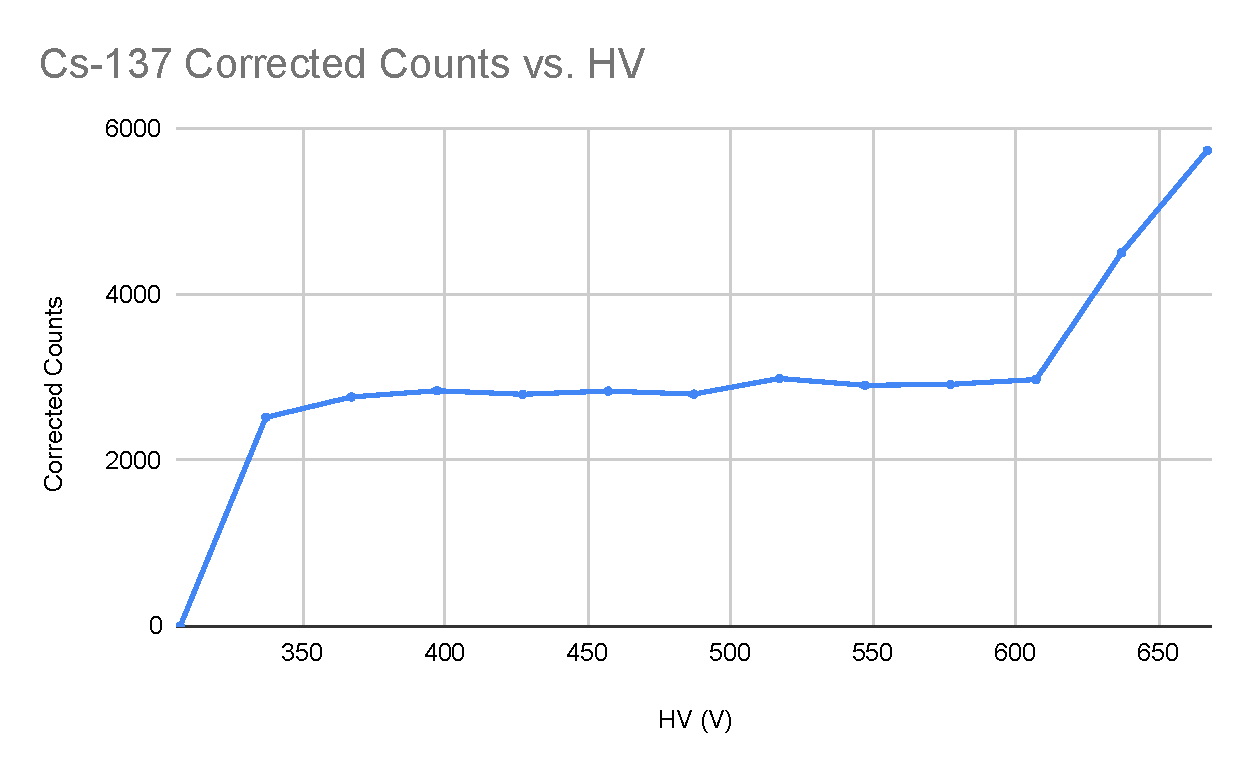
\includegraphics[scale=0.4]{cs1} 
	\caption{GM characteristic curve for Cs-137}
	\label{cs1}
\end{figure}

\begin{figure}[H]
	\centering
	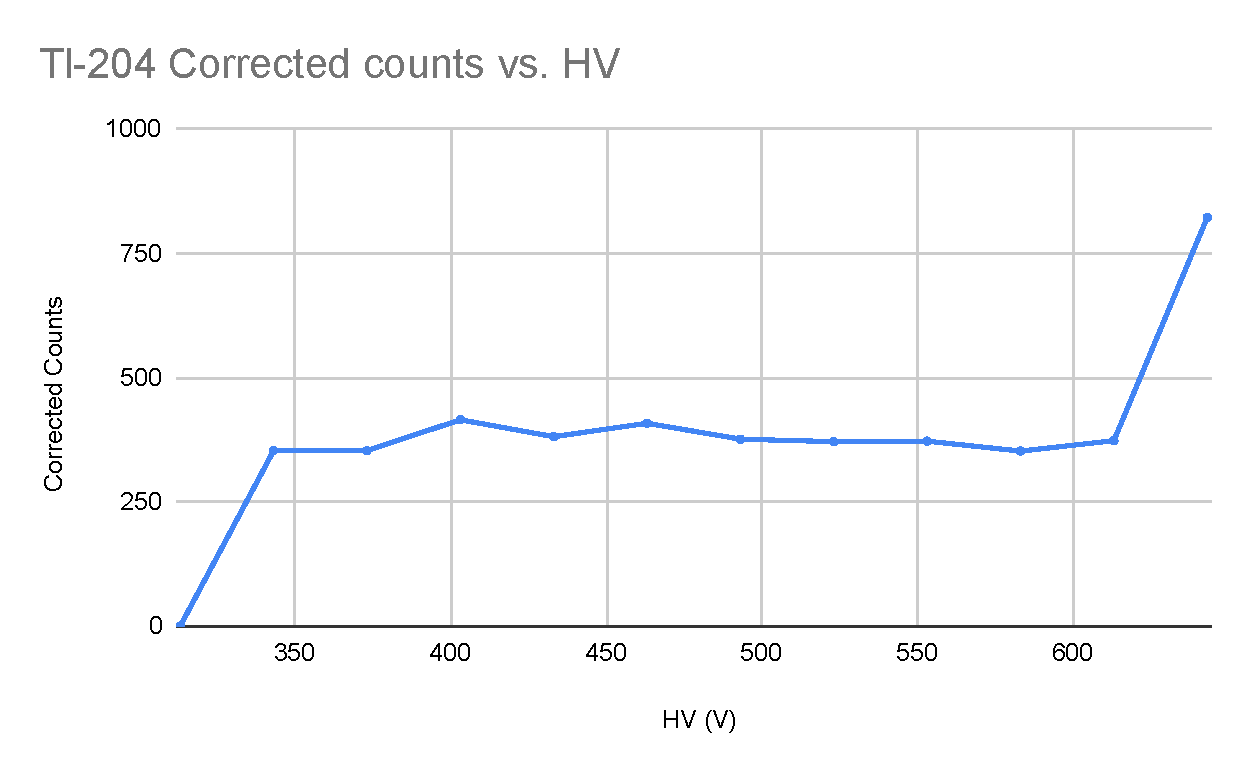
\includegraphics[scale=0.4]{tl1} 
	\caption{GM characteristic curve for Tl-204}
	\label{tl1}
\end{figure}

\subsubsection*{Cs-137}
The starting voltage ($V_1$) is 337 V and Upper threshold voltage ($V_2$) is 607 V. The Plateau length is $V_2-V_1=270~V$. The operating voltage is:
\begin{equation}
	V_o=(V_1+V_2)/2=472~ V
\end{equation}
 The percentage slope of plateau is given by:
 \begin{equation}
 	Slope~Percent=\frac{N_2-N_1}{N_1}.\frac{100}{V_2-V_1}.100
 \end{equation}

where $N_1$, $N_2$ are count rate of  $V_1$ and $V_2$.

 \begin{equation}
	Slope~Percent=\frac{2976-2519}{2519}.\frac{100}{270}.100=6.72\%
\end{equation}

\subsubsection*{Tl-204}

The starting voltage ($V_1$) is 343 V and Upper threshold voltage ($V_2$) is 613 V. The Plateau length is $V_2-V_1=270~V$. The operating voltage is:
\begin{equation}
	V_o=(V_1+V_2)/2=478~ V
\end{equation}

The percentage slope of plateau is given by:
\begin{equation}
	Slope~Percent=\frac{N_2-N_1}{N_1}.\frac{100}{V_2-V_1}.100
\end{equation}

where $N_1$, $N_2$ are count rate of  $V_1$ and $V_2$.

\begin{equation}
	Slope~Percent=\frac{373-353}{353}.\frac{100}{270}.100=2.1\%
\end{equation}

We take operating voltage as mean of both these, i.e 472 V and 478 V giving as 475 V. It is seen that the slope percent less than 10\% is desirable. The mid point of GM characteristics is the operating voltage of the counter. For the beta source the efficiency of detector increases.

\subsection{Inverse Square law} 

The inverse square law states that the intensity of gamma radiation is inversely proportional to the square of the distance of the source.

R is the Net count rate and d is the distance of the source, then:
\begin{equation}
	R=C/d^{2}\implies log(R)=log(C)-2log(d)
\end{equation}
where C is constant.

We can verify the inverse square law by:
\begin{enumerate}
	\item Plot of $1/d^2$ versus R which should be linear
	\item Plot of log(d) versus log(R) where slope should be -2.
\end{enumerate}
as shown in figures (\ref{i1}) , (\ref{i2}) and  (\ref{i3}). The observation tables are shown in tables (\ref{ti1}) and (\ref{ti2}).

\begin{table}[H]
	\centering
	\caption{The mean count is 77.8 with net count rate as 1.3 cps}
	\label{ti1}
	\resizebox{59}{!}{%
		\begin{tabular}{|r|}
			\hline
			\multicolumn{1}{|l|}{Background Count} \\ \hline
			84                                     \\ \hline
			67                                     \\ \hline
			75                                     \\ \hline
			77                                     \\ \hline
			86                                     \\ \hline
		\end{tabular}%
	}
\end{table}


\begin{table}[H]
	\centering
	\caption{Table for inverse square law dependence of intensity with distance.}
	\label{ti2}
	\resizebox{\columnwidth}{!}{%
		\begin{tabular}{|c|c|c|c|c|c|c|}
			\hline
			\multirow{2}{*}{\begin{tabular}[c]{@{}c@{}}Distance\\  d (cm)\end{tabular}} &
			\multirow{2}{*}{\begin{tabular}[c]{@{}c@{}}Corrected \\ Count (N)\end{tabular}} &
			\multirow{2}{*}{Net Count (R)/s} &
			\multirow{2}{*}{$C=Rd^2$} &
			\multirow{2}{*}{$1/d^2 (m^{-2})$} &
			\multirow{2}{*}{log (R)} &
			\multirow{2}{*}{log(d)} \\
			&        &       &        &         &              &              \\ \hline
			2   & 3768.2 & 62.80 & 251.21 & 2500.00 & 1.797982695  & 0.3010299957 \\ \hline
			2.5 & 3011.2 & 50.19 & 313.67 & 1600.00 & 1.700588351  & 0.3979400087 \\ \hline
			3   & 2368.2 & 39.47 & 355.23 & 1111.11 & 1.596267126  & 0.4771212547 \\ \hline
			3.5 & 2025.2 & 33.75 & 413.48 & 816.33  & 1.528316668  & 0.5440680444 \\ \hline
			4   & 1635.2 & 27.25 & 436.05 & 625.00  & 1.435419628  & 0.6020599913 \\ \hline
			4.5 & 1465.2 & 24.42 & 494.51 & 493.83  & 1.38774566   & 0.6532125138 \\ \hline
			5   & 1306.2 & 21.77 & 544.25 & 400.00  & 1.337858429  & 0.6989700043 \\ \hline
			5.5 & 1008.2 & 16.80 & 508.30 & 330.58  & 1.225395443  & 0.7403626895 \\ \hline
			6   & 927.2  & 15.45 & 556.32 & 277.78  & 1.189022173  & 0.7781512504 \\ \hline
			6.5 & 782.2  & 13.04 & 550.80 & 236.69  & 1.115166561  & 0.8129133566 \\ \hline
			7   & 718.2  & 11.97 & 586.53 & 204.08  & 1.07809415   & 0.84509804   \\ \hline
			7.5 & 605.2  & 10.09 & 567.38 & 177.78  & 1.003747669  & 0.8750612634 \\ \hline
			8   & 581.2  & 9.69  & 619.95 & 156.25  & 0.9861743552 & 0.903089987  \\ \hline
			8.5 & 507.2  & 8.45  & 610.75 & 138.41  & 0.9270279945 & 0.9294189257 \\ \hline
			9   & 406.2  & 6.77  & 548.37 & 123.46  & 0.8305886687 & 0.9542425094 \\ \hline
			9.5 & 372.2  & 6.20  & 559.85 & 110.80  & 0.7926251184 & 0.9777236053 \\ \hline
			10  & 360.2  & 6.00  & 600.33 & 100.00  & 0.7783924581 & 1            \\ \hline
		\end{tabular}%
	}
\end{table}

\begin{figure}[H]
	\centering
	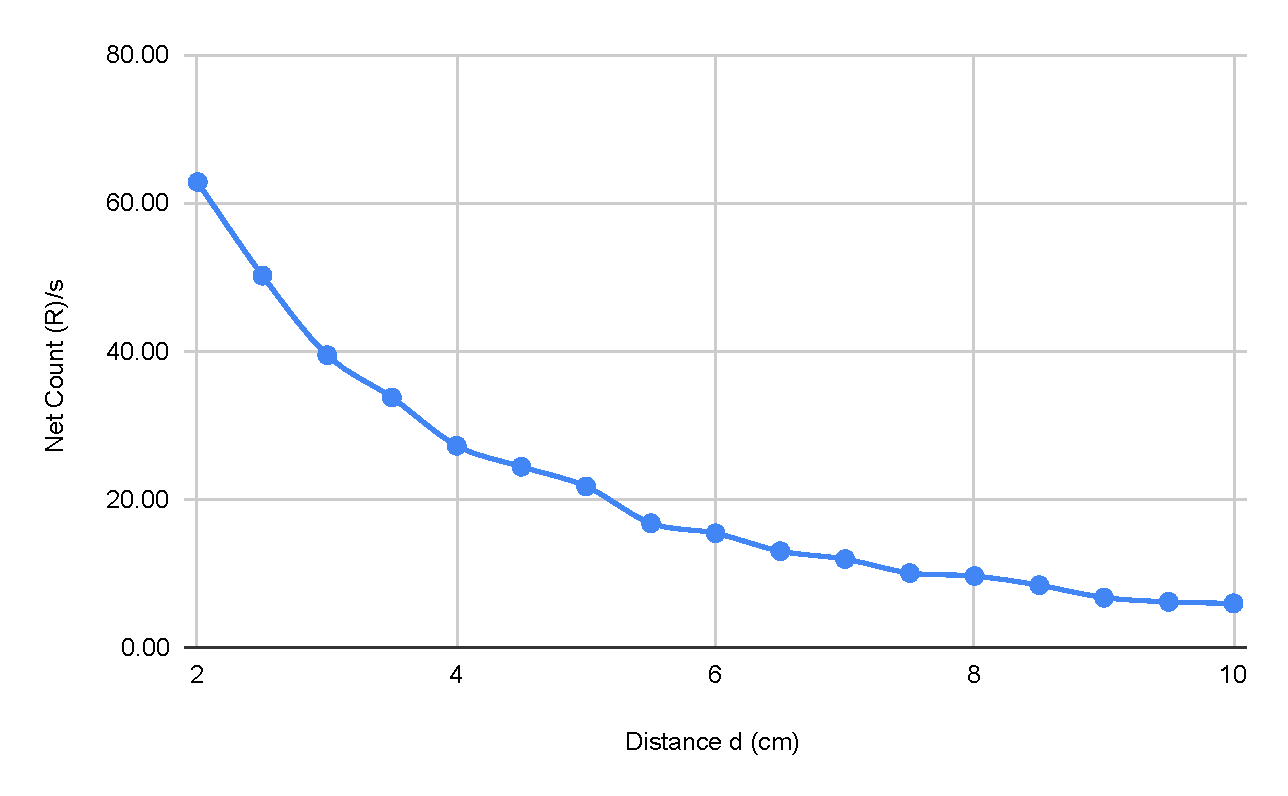
\includegraphics[scale=0.4]{i1}
	\caption{Inverse square law dependence of intensity with distance.}
	\label{i1}
\end{figure}

\begin{figure}[H]
	\centering
	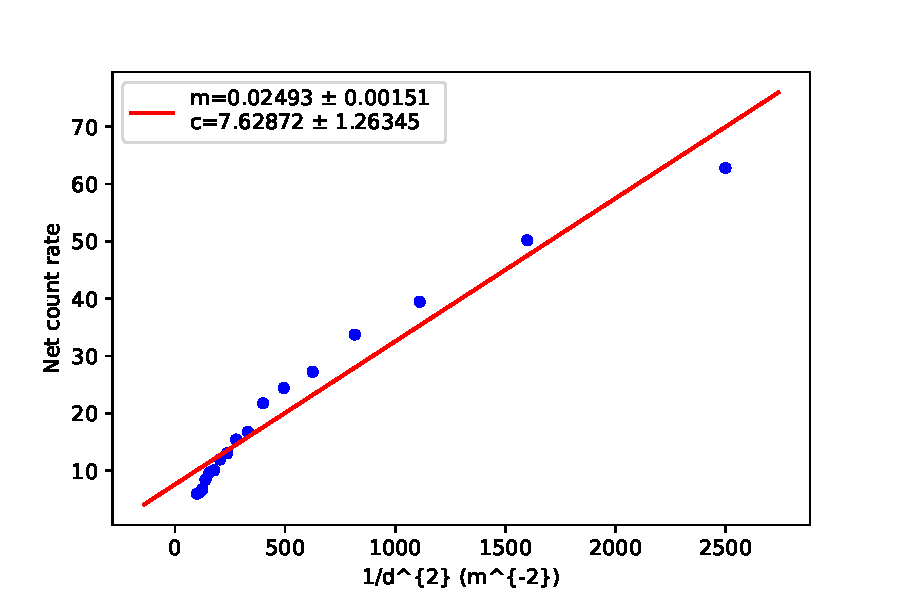
\includegraphics[scale=0.5]{i2}
	\caption{Plot of Net count rate versus $1/d^2$}
	\label{i2}
\end{figure}

The slope of figure(\ref{i2}), gives the value of constant C as $(0.02493\pm0.00151) $ $cps/m^2$. The actual mean and standard deviation of C from the data is $(0.0501\pm0.0109)$ $cps/m^2$.

\begin{figure}[H]
	\centering
	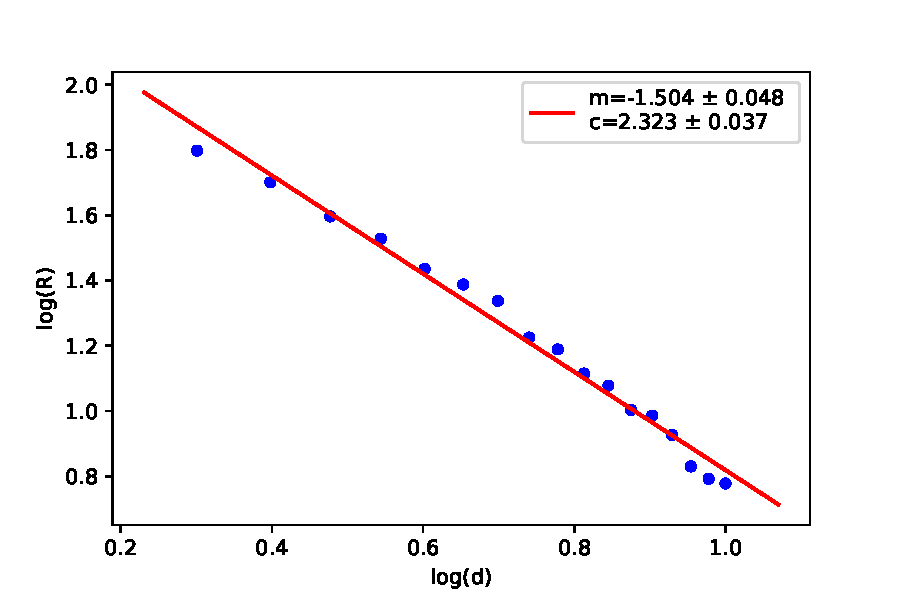
\includegraphics[scale=0.5]{i3}
	\caption{Plot of log(R) and log(d)}
	\label{i3}
\end{figure}

From figure (\ref{i3}), we get slope as (-1.504$\pm$0.048), we expected slope of -2 for inverse square law dependence.


\subsection{Efficiency}
To determine efficiency we need the values of certain parameters which are :
\begin{enumerate}
	\item D, distance of source to end window
	\item d, diameter of end window
	\item $N_s$ mean count due to source
	\item $N_b$ mean count due to background 
	\item A, Activity of the sample.
\end{enumerate}

The D is found to be 10 cm and d is 1.5 cm. Note that cps is counts per second and dps is disintegration per second.

\subsubsection{Cs-137}
The activity A of Cs-137 is 86 kBq.

\begin{table}[H]
	\centering
	\caption{Background count and count recording for 100 s for Cs-137}
	\label{te1}
		\begin{tabular}{|r|r|}
			\hline
			\multicolumn{1}{|l|}{\begin{tabular}[c]{@{}l@{}}Background \\ Count\end{tabular}} & \multicolumn{1}{l|}{Count} \\ \hline
			118 & 438 \\ \hline
			132 & 786 \\ \hline
			116 & 718 \\ \hline
		\end{tabular}
\end{table}

The $N_b=122$ and $N_s=647.3$. Therefore net count rate (N) is 
\begin{equation}
N=(N_s-N_b)/100=5.253~cps
\end{equation}

The gamma source emits radiation in all the directions. The fraction of radiation entering the GM tube is R:
\begin{equation}
	R=\frac{Ad^{2}}{16D^2}=\frac{86000*(1.5)^{2}}{16*10^2}=120.9375~dps
\end{equation}

Therefore, efficiency (E) is 
\begin{equation}
	E=\frac{N}{R}=5.253/120.9375= 4.34\%
\end{equation}


\subsubsection{Tl-204}
The activity of beta source is 10 kBq. We calculate the intrinsic efficiency where geometry factor is not considered for case of beta source.

\begin{table}[H]
	\centering
	\caption{Background count and count recording for 100s for Tl-204}
	\label{te2}
		\begin{tabular}{|r|r|}
			\hline
			\multicolumn{1}{|l|}{\begin{tabular}[c]{@{}l@{}}Background \\ Count\end{tabular}} & \multicolumn{1}{l|}{Count} \\ \hline
			74 & 2454 \\ \hline
			69 & 2498 \\ \hline
			89 & 2493 \\ \hline
		\end{tabular}	
\end{table}

The $N_b=77.33$ and $N_s=2481.67$. Therefore net count rate (N) is 
\begin{equation}
	N=(N_s-N_b)/60=40~cps
\end{equation}

Intrinsic efficiency (E) is calculated as  
\begin{equation}
	E=\frac{N}{A}=0.4\%
\end{equation}


\subsection{Nuclear Counting Statistics}

Systematic errors are precise but not accurate whereas random error lacks precision but not accuracy. Random errors are statistical fluctuations during measurement. The following statistical quantities are defined to know about the data and analyse it.

Mean ($\bar{N}$) is the average value of n measurements,
\begin{equation}
	\bar{N}=\frac{N_1+N_2+.....N_n}{n}
\end{equation}

The deviation ($d$) is the difference between actual value and mean.
\begin{equation}
	d_i=N_i-\bar{N}
\end{equation}

Variance ($\sigma^2$) is the spread between numbers in data. The standard deviation ($\sigma$) is given by square root of variance. 
\begin{equation}
	\sigma^2=\frac{1}{n-1}\Sigma_i^n d_i^2
\end{equation}

For Poisson distribution, variance is equal to mean, i.e $\sigma^2=\bar{N}\implies \sigma =\sqrt{\bar{N}}$

The observation table for this part is attached with the report.

The background count was taken 10 readings for 10 s and 100 s. The bar graph of index versus counts is shown in figures (\ref{10}) and (\ref{100}).

\begin{figure}[H]
	\centering
	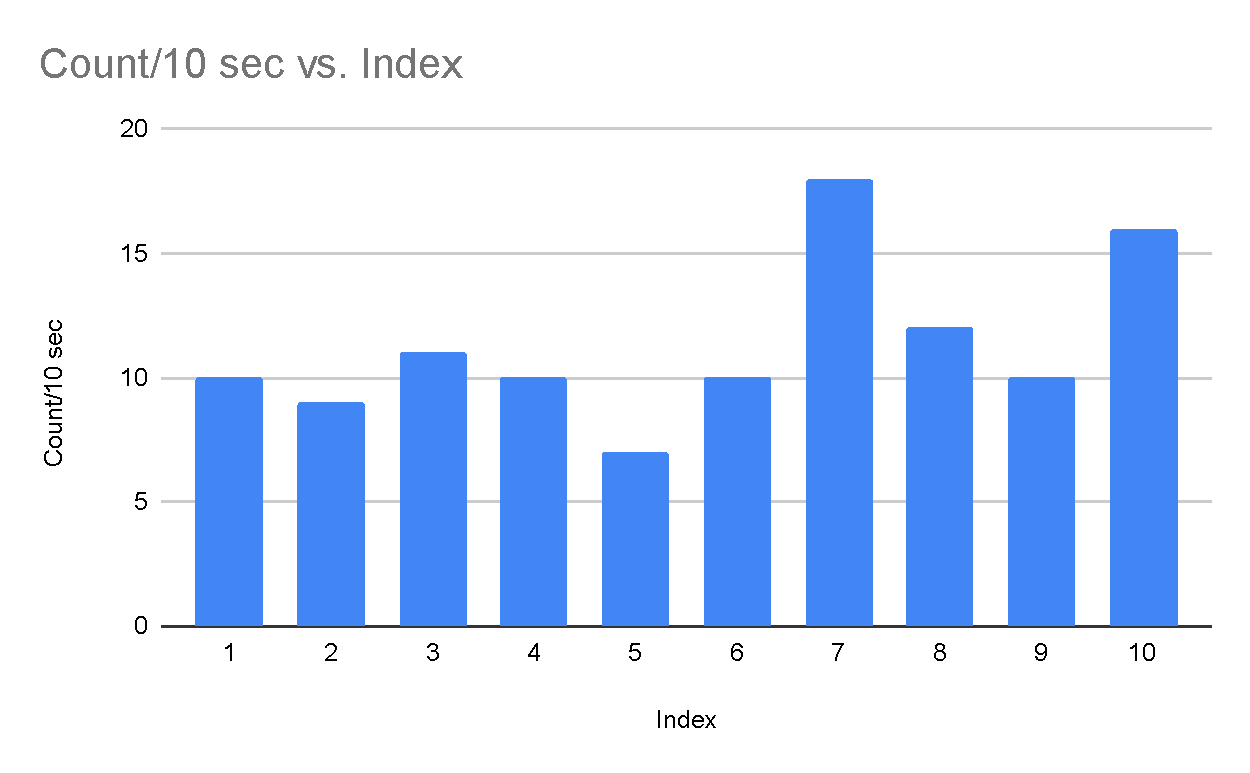
\includegraphics[scale=0.4]{10} 
	\caption{Bar graph of index versus Count for 10 s}
	\label{10}
\end{figure}

\begin{figure}[H]
	\centering
	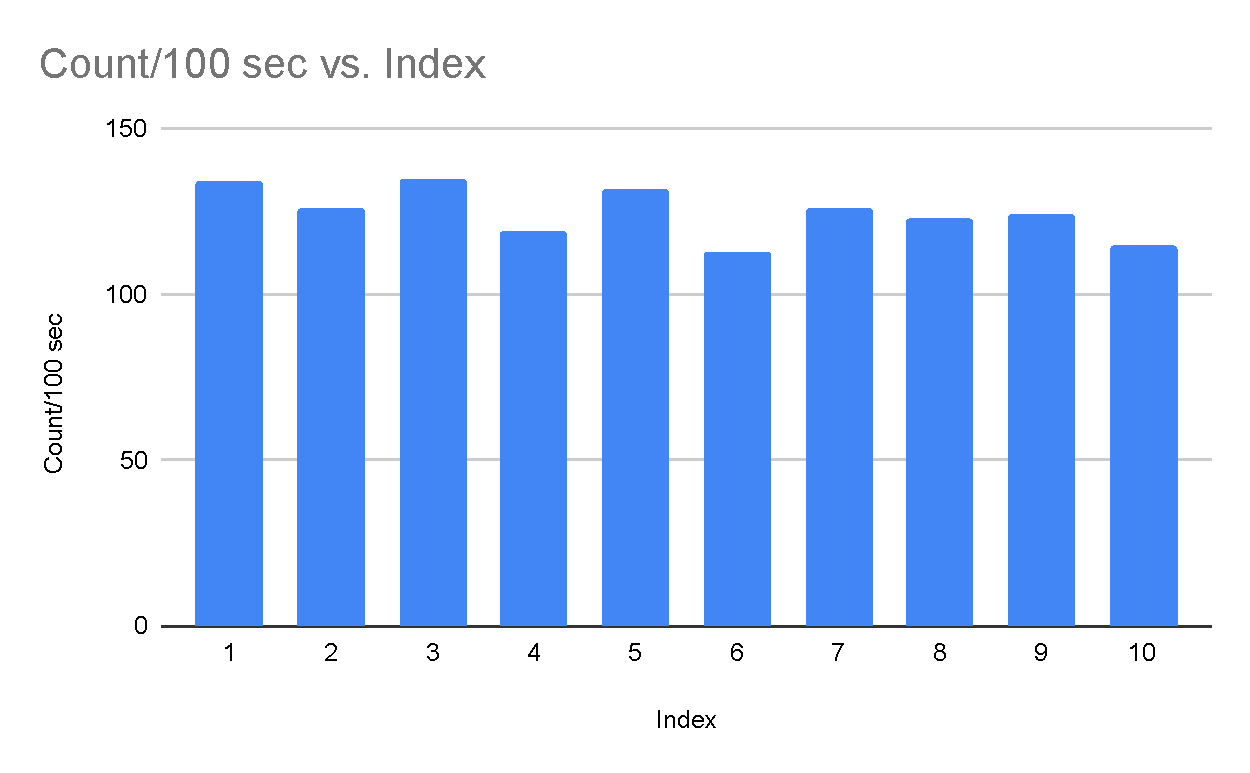
\includegraphics[scale=0.4]{100} 
	\caption{Bar graph of index versus Count for 100 s}
	\label{100}
\end{figure}
 The spread in measure values decreases as number of pulses registered increases.
 
 With 100 readings for 100 s, we obtain mean as 58.55 and variance as 
 \begin{equation}
 	\sigma^2=4774.75/100=47.74
 \end{equation}

Standard deviation $\sigma$=6.90. The histogram of this is shown in figure (\ref{h1}).

\begin{figure}[H]
	\centering
	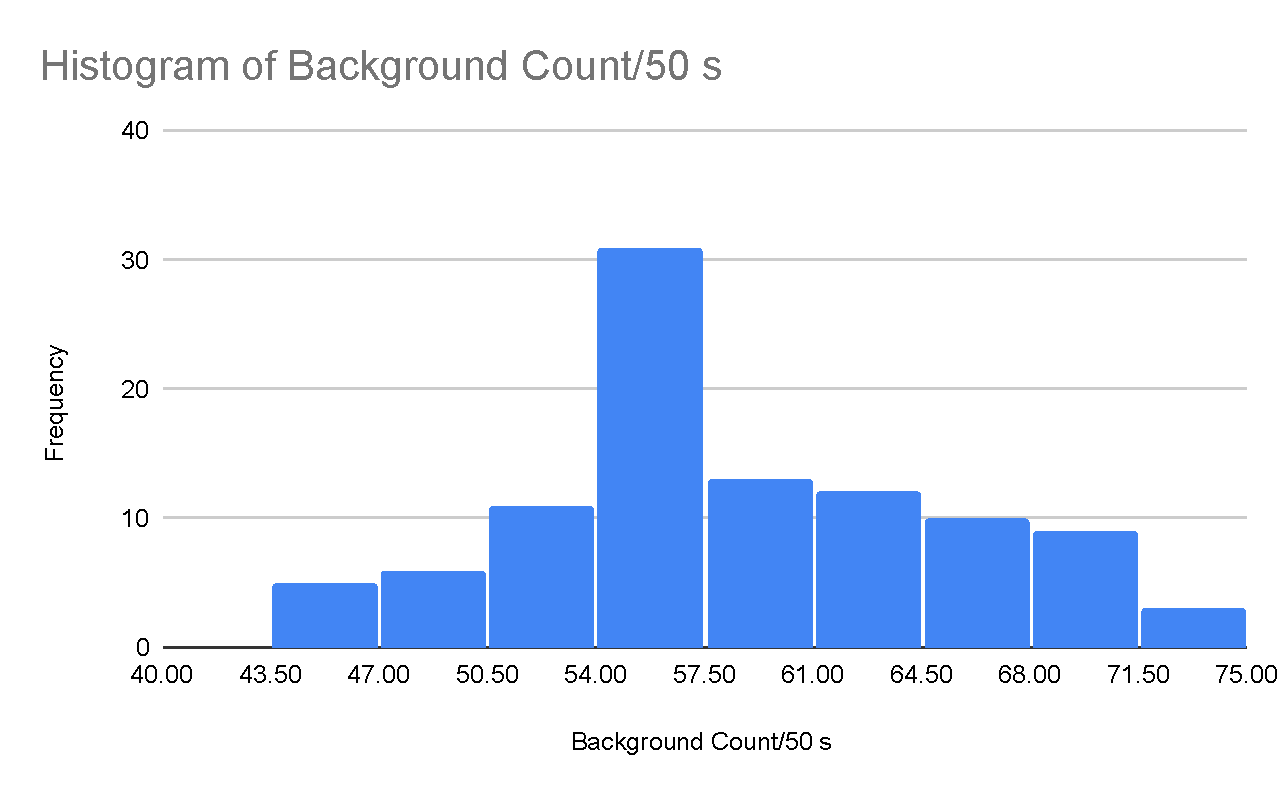
\includegraphics[scale=0.4]{50} 
	\caption{Histogram of Background count in 50 s}
	\label{h1}
\end{figure}

To illustrate the no. of counts being high, Poisson distribution follows Gaussian, we take 50 readings of 25 s with beta source.

\begin{figure}[H]
	\centering
	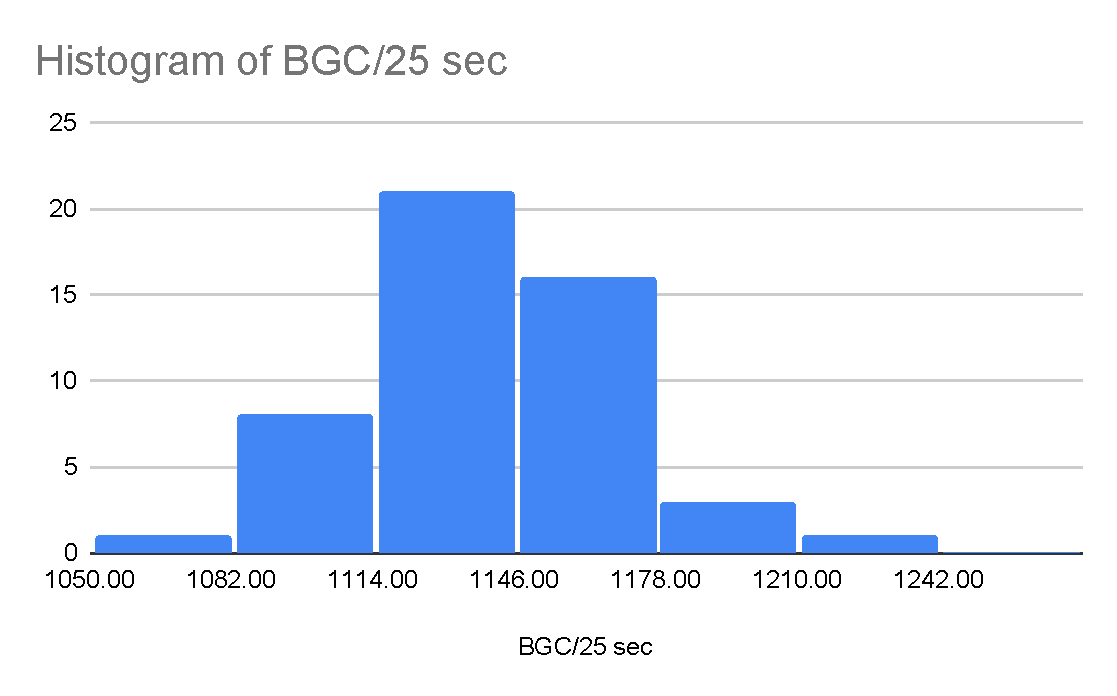
\includegraphics[scale=0.4]{25} 
	\caption{Histogram of count in 25 s with beta source}
	\label{25}
\end{figure}

The mean is 1136.76 with summation of $N_i-\bar{N}$=0.28$\approx$0. The standard deviation is 33.716. It is seen that the histogram of rounded off values is an Gaussian distribution as shown in figure (\ref{d}) and (\ref{r})

\begin{figure}[H]
	\centering
	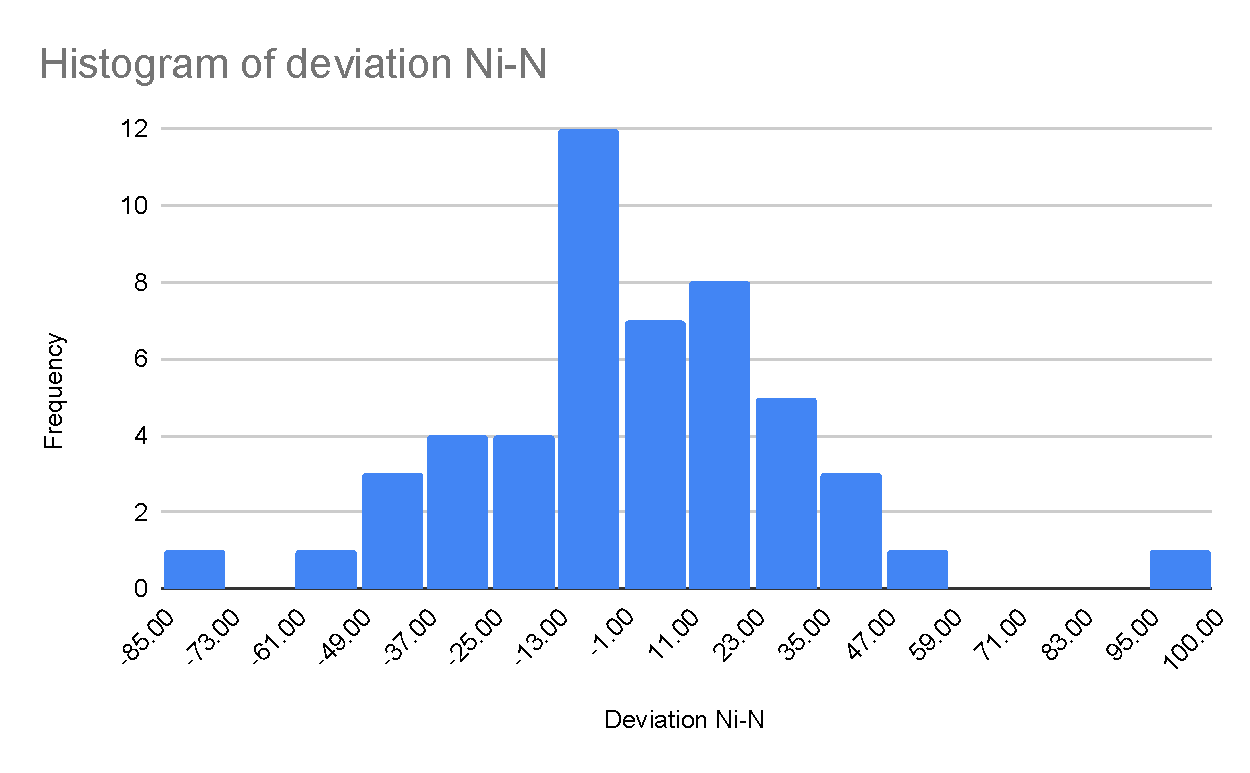
\includegraphics[scale=0.4]{dev} 
	\caption{Histogram of Deviation from the mean}
	\label{d}
\end{figure}

\begin{figure}[H]
	\centering
	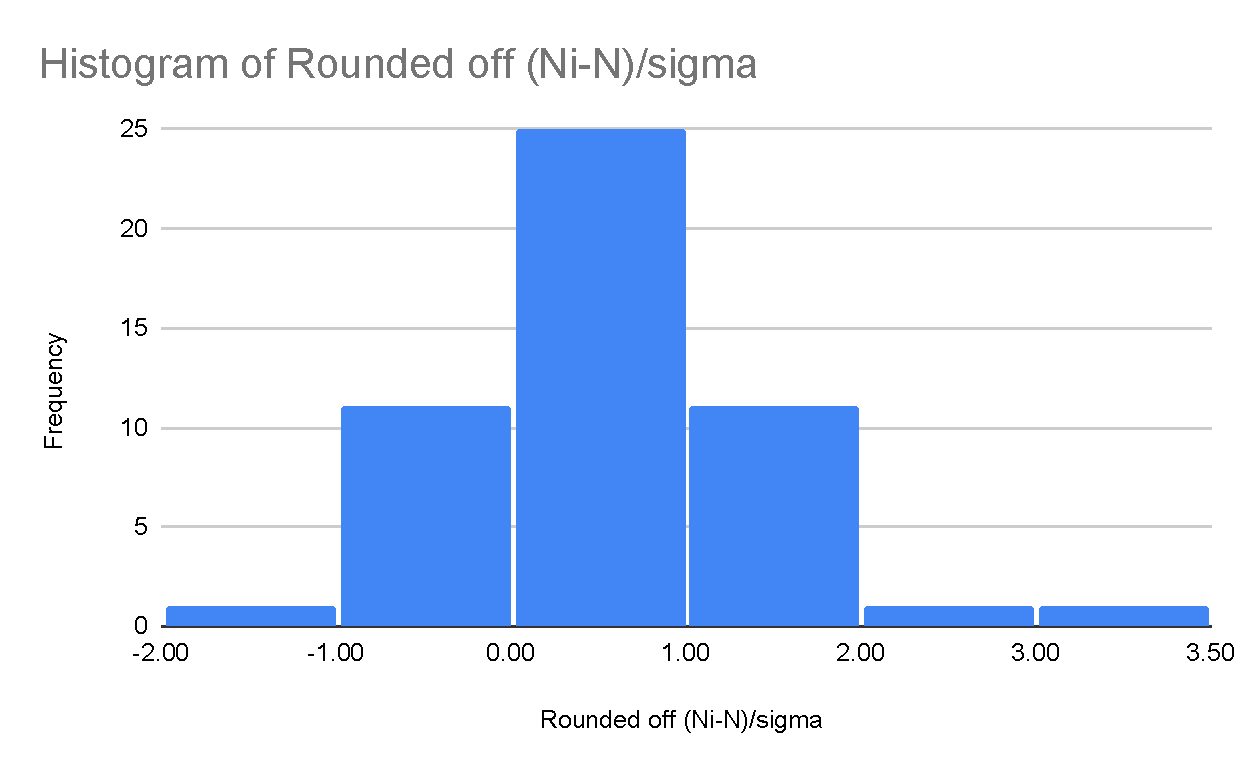
\includegraphics[scale=0.4]{round} 
	\caption{Histogram of rounded off Deviation/standard deviation}
	\label{r}
\end{figure}

\section{Conclusion}
This experiment helped us to familiarize with the basic instrument of nuclear physics lab GM counter. The GM characteristic curve is plateau shaped. The mean of the starting voltage and upper threshold voltage is operating voltage of the counter. We determined the Operating voltage of GM counter as 475 V with slope of plateau as 6.72\% for Cs-137 and 2.1\% for Tl-204. We also verified the inverse square law. We obtained slope from R versus $1/d^2$ as $(0.02493\pm0.00151) $ $cps/m^2$ and the value from data is $(0.0501\pm0.0109)$ $cps/m^2$. We obtained slope as (-1.504$\pm$0.048) while it was expected to be -2 from the plot of log(R) versus log(d) . The efficiency of for gamma source is 4.34\% and beta source is 0.4\%. We also calculated various statistical parameters in the last section. It was seen that mean value is nearly same as variance, which is Poisson distribution. The distribution around the mean value closely resembles to Gaussian. Some of the errors may have contributed to the experiment. This included the systematic error in the GM counter as the timer lagged than the original timer. Moreover the value could be made precise by increasing number of readings.

\section{References}
\begin{enumerate}
\item{\url{https://www.imagesco.com/geiger/geiger-counter-tube.html}}
\item{\url{https://www.niser.ac.in/sps/sites/default/files/basic_page/p341_2023/GM-1.pdf}}

\end{enumerate}

\end{document}